\documentclass{amsart}
\usepackage[usefamily=sage]{pythontex} 
%\usepackage{sagetex} 
\usepackage{float}
\usepackage{tikz}
\usetikzlibrary{calc}
\usepackage[utf8]{inputenc}
\usepackage[most]{tcolorbox}
\usepackage[margin = 2cm]{geometry}

\newtheorem{ejer}{Ejercicio}
\def\r{\mathbb{R}}
\title{Tarea 08. Giros en el Plano \\ AMD 2023-24}

\begin{document}
\maketitle

\begin{ejer}
Construye la bandera de Chile con la especificaciones indicadas el el siguiente gráfico:

\begin{figure}[H]
\centering
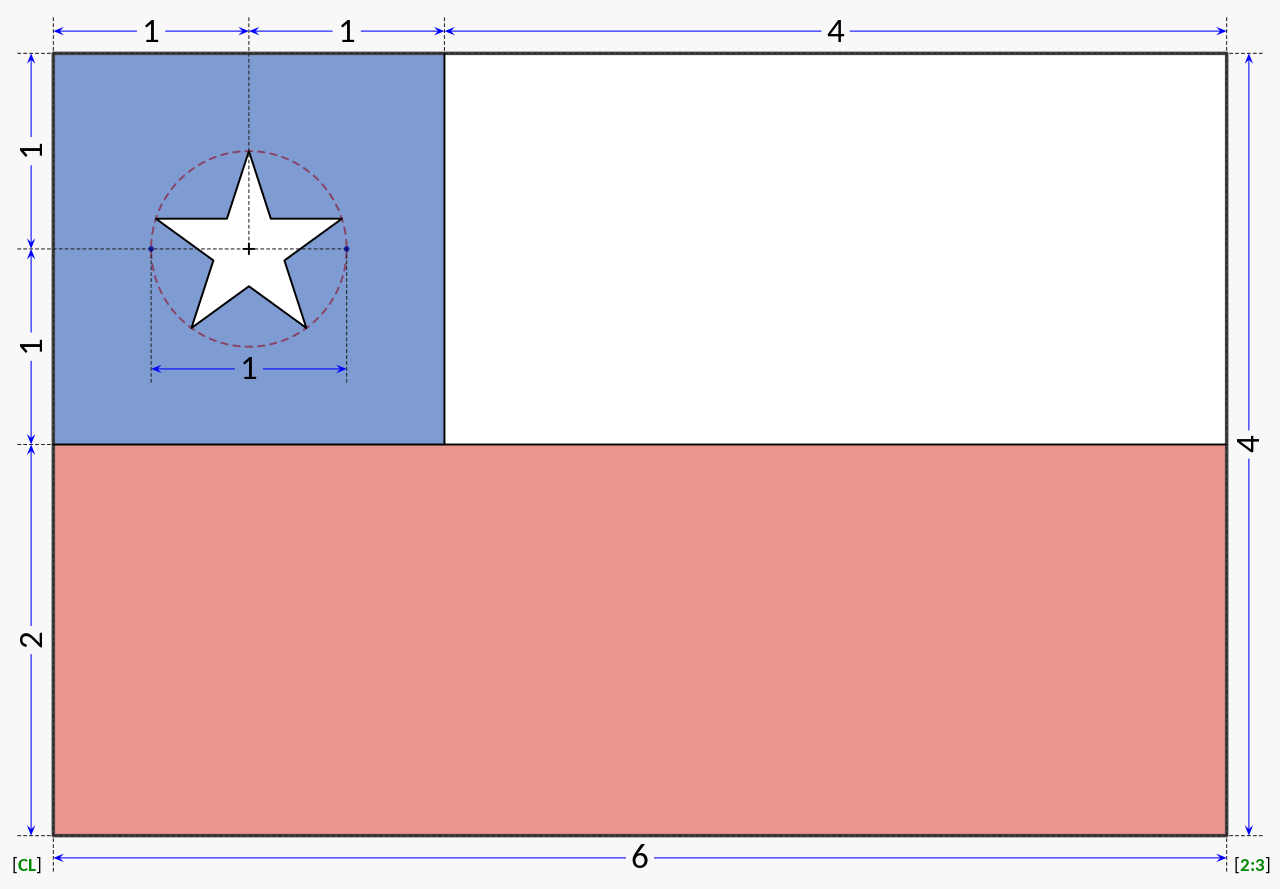
\includegraphics[width = 12cm]{Chile.png}
%(Fuente: \url{https://en.wikipedia.org/wiki/Flag_of_Chile#/media/File:Flag_of_Chile_(construction_sheet).svg})
\end{figure}
\end{ejer}

{\it Solución:}

% Escribe tu solución para el ejercicio 4

\begin{sageblock}
A = vector([0,0])
B = vector([6,0])
C = vector([6,2])
D = vector([6,4])
E = vector([2,4])
F = vector([0,4])
G = vector([0,2])
H = vector([2,2])
\end{sageblock}

\begin{sagesub}
	\begin{center}
		\begin{tikzpicture}[x = 0.25cm, y = 0.25cm]
			\node (A) at !{A} {$A$};
			\node (B) at !{B} {$B$};
			\node (C) at !{C} {$C$};
			\node (D) at !{D} {$D$};
			\node (E) at !{E} {$E$};
			\node (F) at !{F} {$F$};
			\node (G) at !{G} {$G$};
			\node (H) at !{H} {$H$};
			\draw (A) -- (B) -- (D) -- (F) -- (A);
		\end{tikzpicture}
	\end{center}
\end{sagesub}

\end{document}
